\section{Kosten}



\subsection{Betriebskosten}

Die Betriebskosten bei einer Flugzeugabfertigung werden auf Direct Operating Costs (DOC), und Indirect Operating Costs 
(IOC) geteilt, die werden auch Einzel- und Gemeinkosten genannt \cite{conrady2019luftverkehr}. 
DOC können einem bestimmten Flugzeug oder einer Strecke zugeordnet 
werden und können normalerweise als DOC pro Flugstunde, DOC/Kilometer, DOC/Passagierkilometer oder DOC/Blockstunde 
berechnet werden \cite{mensen2013handbuch}. 
Wobei IOC sind nicht direkt einem Flug zugewiesen, sondern für den gesamten Betrieb anfallen, wie z.B. zeitabhängige 
Instandhaltungskosten, Verwaltungskosten, Infrastrukturkosten \cite{mensen2013handbuch}. 

Nach der Beschäftigungsabhängigkeit werden die Kosten auf fixe und variable Kosten aufgeteilt. 
Fixe Kosten sind unabhängig von dem Betrieb (z.B. Kapitalkosten, Versicherung, Personalkosten), 
wo hingegen die variablen Kosten sind von der Beschäftigung ändern \cite{mensen2013handbuch}.



Die Struktur der Kosten einer Fluggesellschaft kann mit der folgenden Abbildung veranschaulicht werden.

\begin{figure}[h]
	\centering
	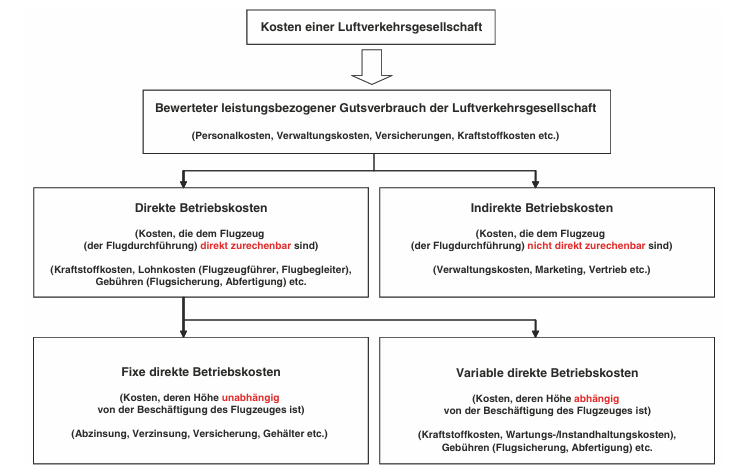
\includegraphics[width=0.9\linewidth]{Bilder/Systematik der DOC_Berechnung.png}
	\caption[DOC]{ \cite{mensen2013handbuch}}
	\label{doc}
\end{figure}


Betriebskosten sind von dem Flugzeug abhängig, deswegen ist es wichtig vor der Anschaffung zu überprüfen, 
ob es ein Flugzeug mit alternativem Antrieb rentabel ist. Die neuen Regularien für \ce{CO2}-Reduktion können einen Anreiz oder sogar 
eine Verpflichtung für die Fluggesellschaften schaffen, um die beste Lösung für eine Flotte zu finden. Mehr um politische Anreize gibt es im Kapital.

Fuel, Technikkosten (Wartung, Reparatur, Instandhaltung MRO) - es gibt unterschiedliche Typen von Wartung, die Kontrolle was am Vorfeld bei einem 
Turnaround passiert ist die line maintenance (prüfung von Reifendruck und Ölständen), Flughafenentgelte und Handlingkosten: 
Bodenabfertigung besteht aus Passagierabfertigung, Fracht-, Gepäckabfertigung und VorfelddiensteFlugzeugabfertigung ist direkte Kosten, 
Passagierkosten indirekte Kosten, Kapital- und Abschreibungskosten \cite{conrady2019luftverkehr}. 
Conrady bescheibt die Cockpit Crew als auch Cabin Crew, so Gehälter, Reisekosten, Schulungskosten. Es gibt jedoch nur wenige Arbeiten, 
die die Ausbildungskosten erwähnen. Auch Handling Agents Kosten gibt es nicht viel Information zu finden. Es kann damit zurückgeführt werden, dass
sind unabhängige von Fluggesellschaften Handling Agents für Abfertigung zuständig und nicht die Fluggesellschaften Kosten dafür übernehmen.

92 Milliarden Gallonen Kraftstoff wurden durch der Luftfahrindustrie im Jahr 2023 verbraucht.\cite{iata_industry_statistics_2024}
Kesorinpreis im Jahr 2022 betrug USD 136/bbl (ca. 133€/bbl Wechelkurs 14.01.25 \cite{ecb_exchange_rates_usd}
Der Treibstoffrechnung war fast 32\% alles Betriebskosten in der Luftfahrt im Jahr 2023. \cite{iata_industry_statistics_2024}

Wartungskosten sind von Auslastung eines Flugzeugs, je schnellere Wartung man braucht, desto teurere Komponente man braucht.

Die Kurzstrecken-Flugzeuge sind mehr mit größerer Anzahl an Landungsgebühren und größere Treibstoffverbrauch verbunden sind, da 
der Start und die Landung sind die Treibstoff aufwendigste Prozesse im ganzen Flug.

Für Szenarien Flottenabhängigkeit: Je mehr die gleichen Flugzeuge-Typen, desto geringere Wartungskosten zu erwarten.


In den USA ein Drittel von allen Gesamtkosten (TOC) aller Fluggesellschaften sind die Kosten für Treibstoff und Öl 
und ein Sechstel ist die Abfertigung am Flughafen \cite{conrady2019luftverkehr}. 

%Eine Reihe anderen Kosten, die für die Arbeit vielleicht nicht relevant?: Flugsicherungsgebühren, Versicherungskosten (bleiben), 
%Servicekosten, Marketing- und Vertriebskosten, Kpsten der allgemeinen Verwaltung, 
Diese werden aufgrund der Komplexität der Berechnungen und der begrenzten Verfügbarkeit von Daten nicht weiter betrachtet.
Cockpit crew and cabin crew Kosten bestehen aus Gehälter, Reisekosten und Schulungskosten \cite{conrady2019luftverkehr}.

"Zu den direktenvariablenKosten (flugereignisabhängige Kosten) zählen– Abfertigungsentgelte Fluggerät,– Landeentgelte,
– Flugsicherungsgebühren,– Dritthaftpflichtversicherung,– Treibstoff,– Bordservicekosten,– Reisekosten Cockpit/Kabine,
– variableInstandhaltungskosten,– variableFrachtkosten (z.B. für Anlieferung) und– Charterkosten."

"Die direkten Fixkosten (Kapazitätsvorhaltungskosten) umfassen– direktefixeTechnikkosten,– Stationswartung,
– Kapitalkosten Fluggerät,– Leasingkosten Fluggerät,– Zinsen Fluggerät,– Vorlaufkosten Fluggerät,– Versicherungen Fluggerät,
– Personalkosten Cockpit/Kabine und– Trainings-/Vorlaufkosten Cockpit/Kabine."


In den USA ein Drittel von allen Gesamtkosten (TOC) aller Fluggesellschaften sind die Kosten für Treibstoff und Öl 
und ein Sechstel ist die Abfertigung am Flughafen \cite{conrady2019luftverkehr}. 

In dieser Arbeit wird der Fokus auf die direkten Betriebskosten gemacht.




Preis für Treibstoffversorgung für kurzfristige Perioden kann folgend berechnet werden \cite{iata_saf_procurement_2024}: nicht sicher, ob die Formel nehme
PRA-Bewertung (Risikobewertung??? Durchschnitt der Vorperiode) + Logistikkosten + zusätzliche Gebühren + Lieferantenmarge


"Das Schulungsprogramm muss eine Kompetenzschulung für alle installierten Geräte umfassen." (ICAO Annex 6 Teil 2)

(Annex  Doc 1984 Teil 1 Chapter 13 Seite 141)
Bei konventionellen Kraftstoff kann die Logistik mit einem Schiff, Binnenschiff, Bahn, Lkw oder Pipeline durchgeführt. 
Diese Optionen haben große Auswirkungen auf die Kapitalkosten eines Flughafens und müssen sorgfältig berechnet werden. 
eine von spezialen Anforderungen bei Planung von Flughafeninfrastruktur "Minimierung der Belegungszeiten am Flugzeuggate; 
die erforderlichen Kraftstoffdurchflussraten sind ein Faktor bei der Wahl des einzusetzenden Betankungssystems"

Abhängigkeit der Betriebskosten von Treibstoff-Kosten beschreiben.


Abschreibungskosten sind ein Teil der Kapitalkosten für das Flugzeug, die für den festgelegten Zeitraum, wo Flugzeug benutzt wird, verteilt.


%Conceptual_Design_and_Operating_Costs_Evaluation_of_a_19-seat_All-Electric_Aircraft_for_Regional_Aviation
"die Zins- und Abschreibungskosten sinken tendenziell bei hoher Tagesauslastung"
20 Prozent in Motorwartung verringert DOC um 4%


DMC are the maintenance costs caused directly by the aircraft; 
Wartung "line maintenance cost;
periodic maintenance cost;
workshop direct maintenance cost; and
overhaul cost."

\subsection{Infrastrukturkosten}
